% \begin{multicols}{2}
\section{Resultat}

Das Produkt dieser Arbeit ist zum einen die Web-App, welche in allen modernen Webbrowsern funktioniert. Durch Klicken können in der 3-D-Karte Start- \& Zielpunkt ausgewählt werden. Mit einem bestätigenden Mausklick auf <<Ausführen>> wird im Hintergrund ein \gls{gis}-Modell gestartet, welches entweder eine <<rohe>> Gefahrenkarte oder eine mit enthaltenen Gewässern verwendet. Mit eigenen Touren kann auf \url{https://algotour.app} experimentiert werden. (Siehe Abb.\ \ref{fig:mainui})

Zum anderen sind die zugehörigen \acrshort{gis}-Modelle, welche im Hintergrund für alle Berechnungen benötigt werden, ebenfalls Teil des Resultats. Abb.\ \ref{fig:walkmodel} ist ein Beispiel eines solchen Modells. Konkret ist das hier gezeigte Modell für die endgültige Pfadberechnung auf dem Server verantwortlich.

% \skiplines{3}
\begin{figure}[H]
  \centering
  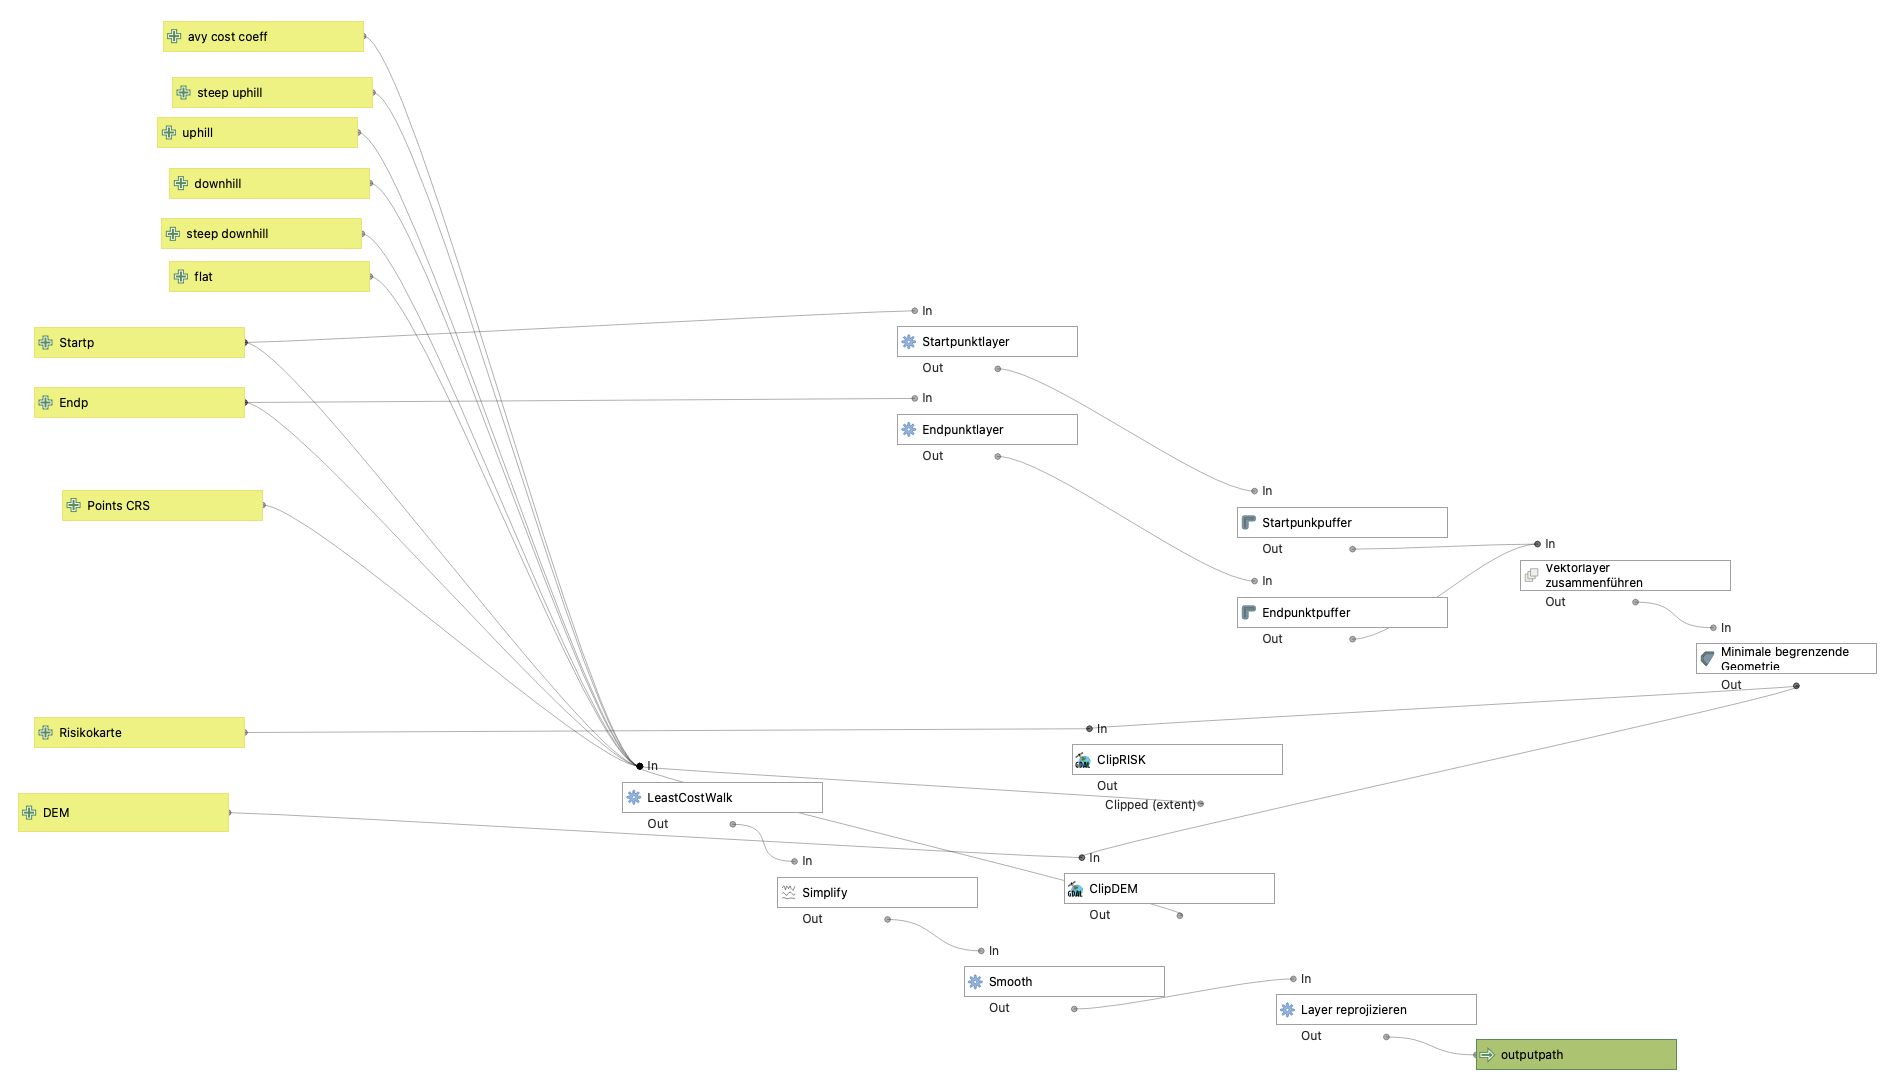
\includegraphics[width=\linewidth]{Modell_Walk.png}
  \caption{Endgültiges Modell zur Berechnung von Touren}\label{fig:walkmodel}
\end{figure}
\begin{figure}[H]
  \centering
  
\includegraphics[width=4cm]{qrlink}
  \caption{QR-Code mit Link zur Web-Applikation}\label{fig:qrlink}
\end{figure}


\clearpage
\section{Diskussion}

\subsection{Modellevaluation}

14 typische Frühlings-Skitouren \& -Skihochtouren wurden aus dem SAC Tourenportal ausgewählt und durch ein kurzes Python-Skript heruntergeladen. Anschliessend wurden die Modellversionen mit und ohne eingebrannten Gewässern für die Start- und Zielpunkte der einzelnen Routensegmente ausgeführt. Start- und Zielpunkte wurden dabei von Hand platziert. Für alle 28 Tests wurden die gleichen Hyperparameter verwendet: \\$k_{risk}={50.0};\ c_{steepascend}={5.0};\ c_{steepdescend}={5.0};\ c_{flat}={0.25};\ c_{ascend}={2.5};\ c_{descend}={2.5}$

Für einige Regionen bzw. Gipfel (Länta, Steingletscher) war nur eine von beiden Gefahrenkarten brauchbar -- so ist es kaum sinnvoll, quer durch den Steinsee zu waten, da dieser nur selten zugefroren ist. Erfahrungswerte mit beiden Modellversionen zeigen, dass der Benutzer in den meisten Fällen beide Versionen begutachten sollte.

Nachfolgend wird eine Auswahl der Touren kurz diskutiert: Die besten Routen waren jene vom Steingletscher aus auf die Tierberglihütte SAC, sowie auf das Sustenhorn, dies unter der Bedingung, dass die korrekte Gefahrenkarte verwendet wird; die andere Risikokarte produziert unbrauchbare Resultate. Es lässt sich eine hohe Übereinstimmung mit den Literatur-Routen, welche der SAC im Tourenportal auflistet feststellen~\cite{mmzentralch} (siehe Abb.\ \ref{fig:tierbergli}).
% \end{multicols}
\begin{figure*}[ht]
  \centering
  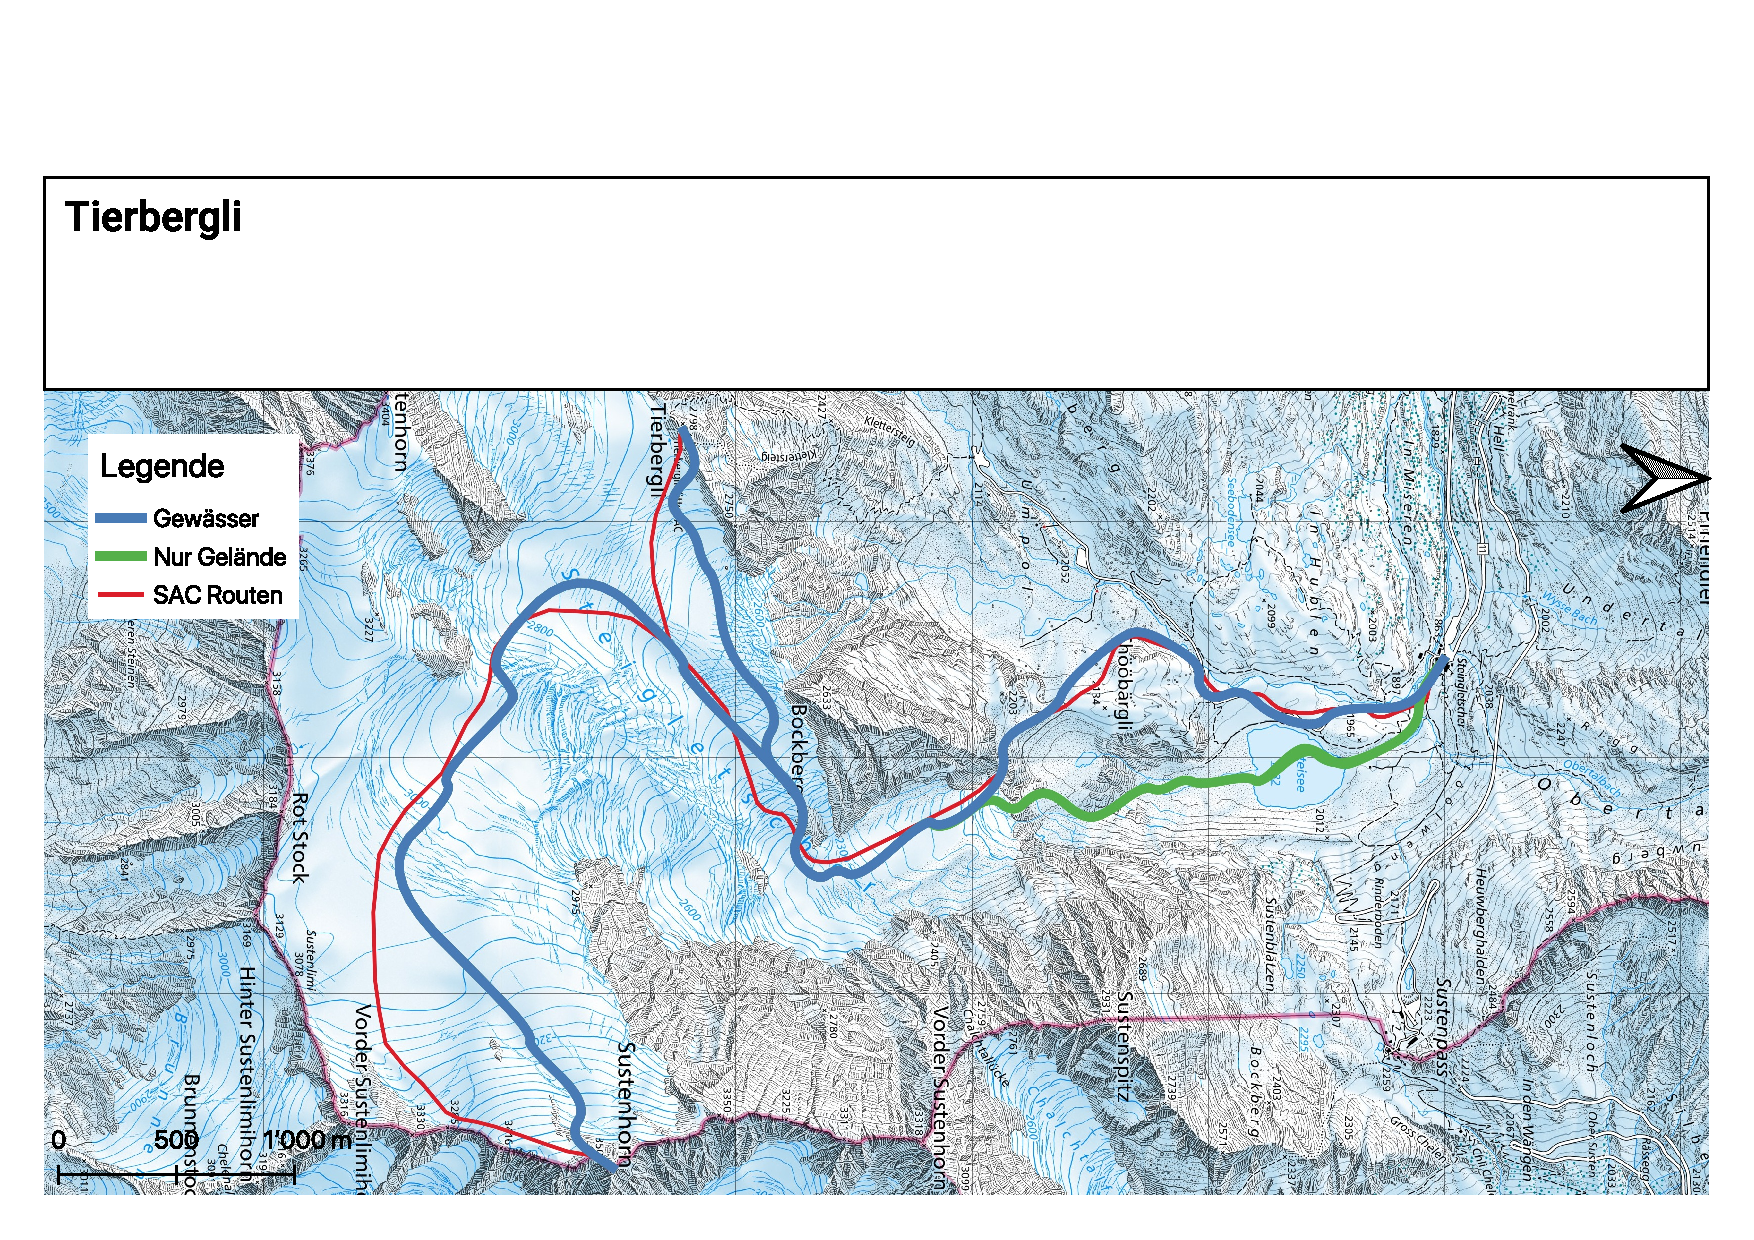
\includegraphics[page=1,width=.9\linewidth]{./../evaluation/PDFs/Tierbergli.pdf}
  \caption{Tour auf Tierberglihütte SAC und Sustenhorn ab Steingletscher, \\Basislayer: swisstopo}\label{fig:tierbergli}
\end{figure*}

% \begin{multicols}{2}

Ebenso erreicht die Tour auf den Clariden in der Eigenevaluation eine Bestnote. Hier trumpft jedoch die nicht mit Gewässern ergänzte Karte (siehe Abb.\ \ref{fig:clariden}). Die nicht ganz offensichtlichen Gratpassagen werden vom Modell sehr gut abgebildet, der Bach wird an einem sinnvollen Ort überquert. Die Übereinstimmung mit der SAC-legitimierten Route ist ebenfalls hervorragend~\cite{twslstgallappzll}.

% % \end{multicols}
\begin{figure*}[ht]
  \centering
  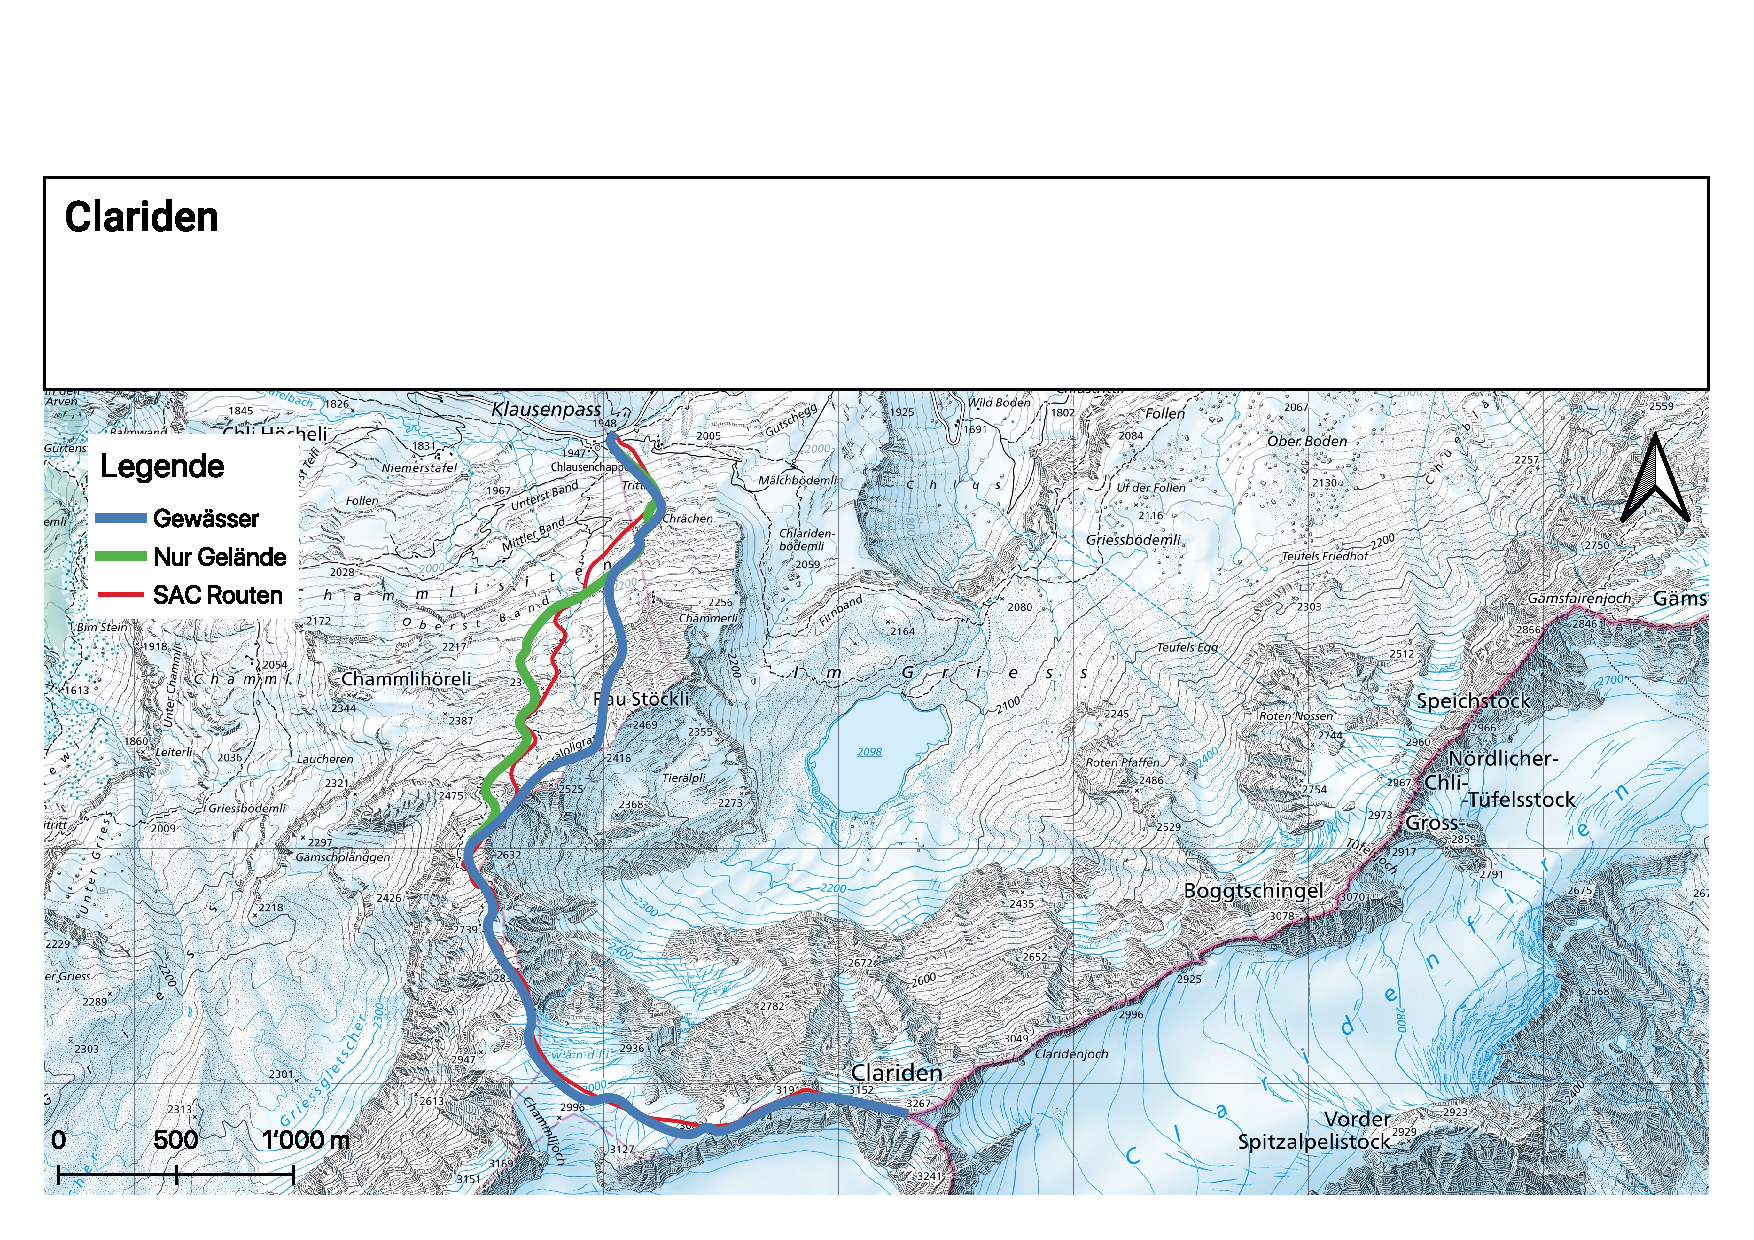
\includegraphics[page=1,width=.9\linewidth]{./../evaluation/PDFs/Clariden.pdf}
  \caption{Geplante Tour von der Klausenpass-Passhöhe auf den Clariden, \\Basislayer: swisstopo}\label{fig:clariden}
\end{figure*}

% % \begin{multicols}{2}

Weniger erfreulich sieht das Resultat bei den Touren im Monte-Rosa-Massiv aus. Bei der Route auf die Dufourspitze findet der Algorithmus ohne weitere Hilfe zwar eine Spuranlage, welche als Hochtour so existiert, im Winter jedoch -- wegen einer Kletterstelle im~\rom{3}. Grad -- kaum oder nur unter extremer Schwierigkeit und nur ohne Skis begangen werden kann. 
Die Tour welche nicht direkt zum Gipfel, sondern nur bis zum Skidepot der Literaturtour führt, funktioniert und kann so begangen werden. Die Routenwahl ist jedoch um einiges defensiver als jene aus dem Tourenführer (siehe Abb.\ \ref{fig:monterosa} <<Manuelles Skidepot>>). Ein Umweg von ca.\ \qty{1}{h} wird gegenüber einem \qty{32}{°} steilen Hang in Kauf genommen.

% % \end{multicols}
\begin{figure*}[ht]
  \centering
  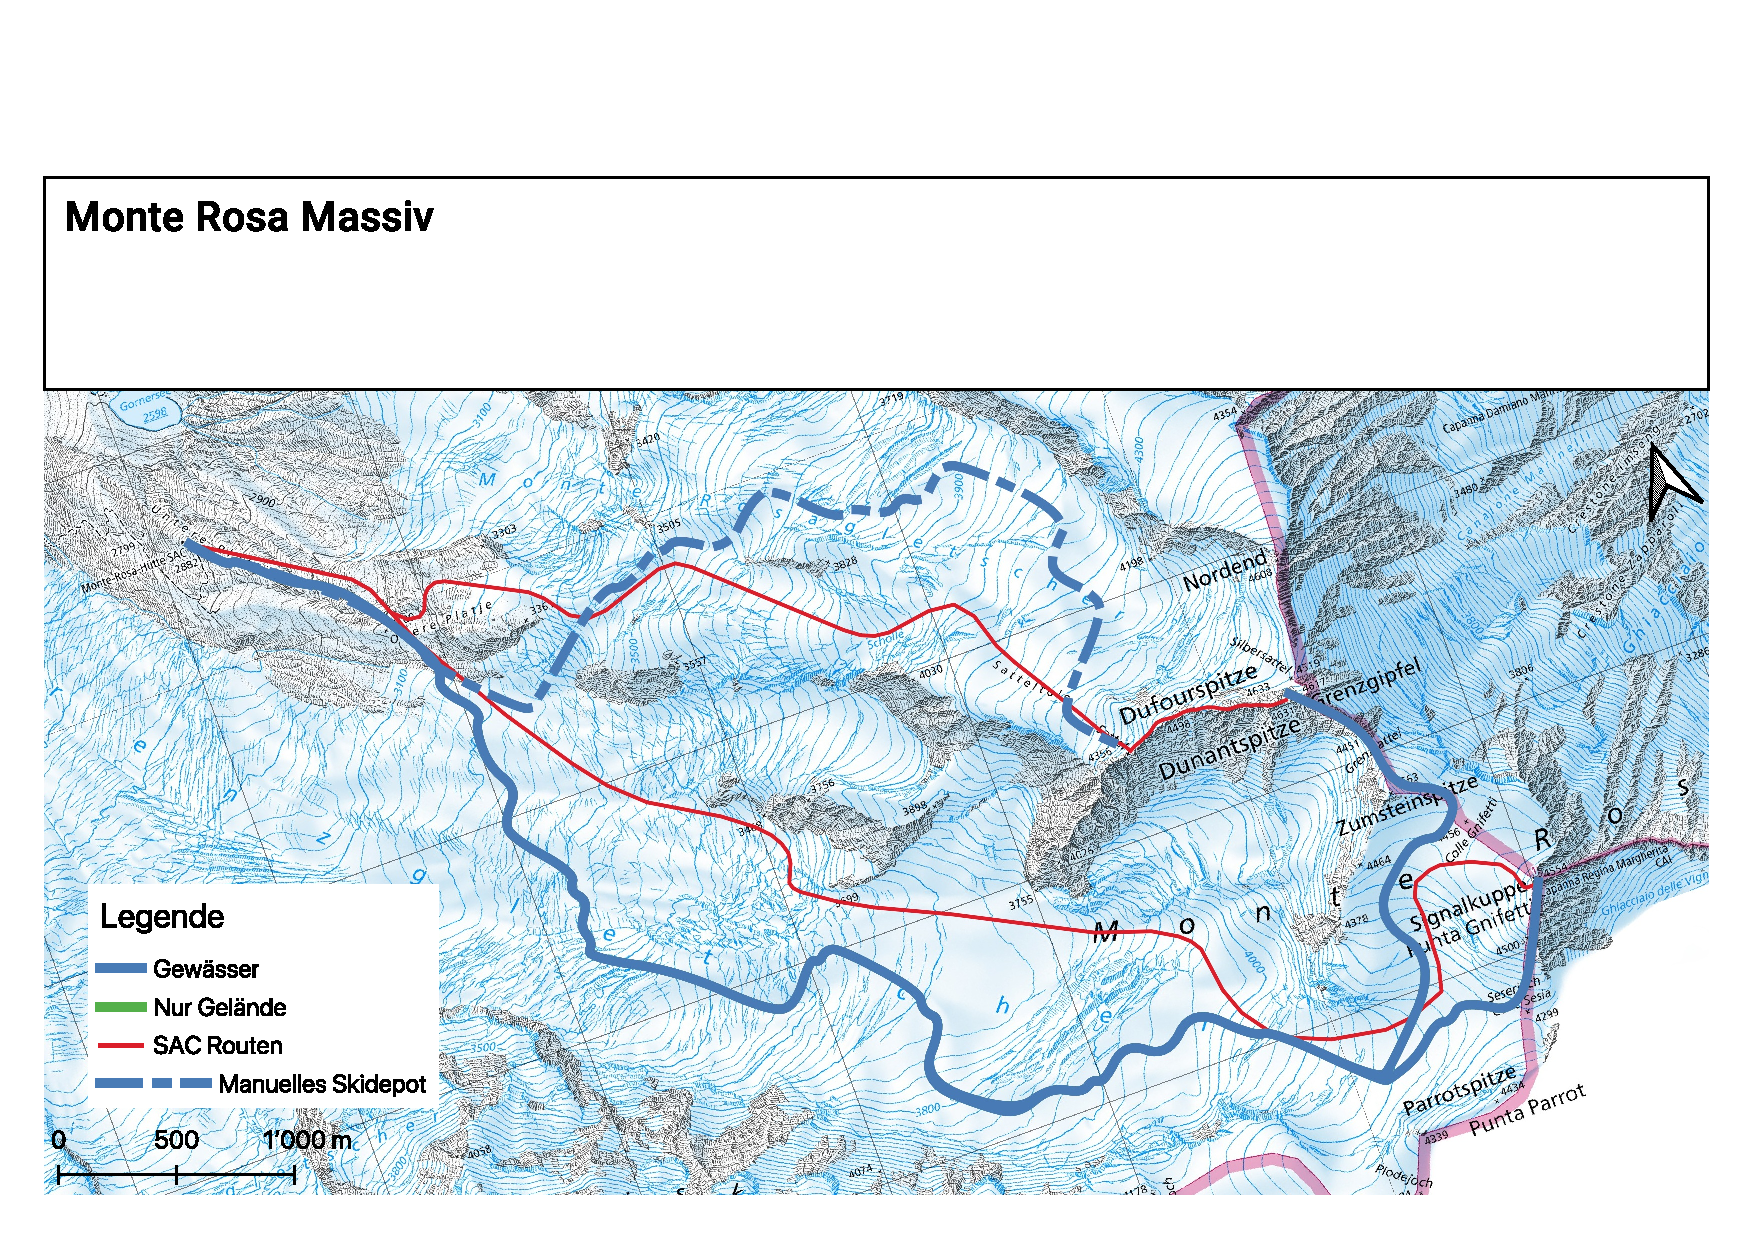
\includegraphics[page=1,width=.9\linewidth]{./../evaluation/PDFs/Monte Rosa Massiv.pdf}
  \caption{Geplante Tour von der Monte-Rosa-Hütte SAC auf Dufourspitze und Signalkuppe,\\Basislayer: swisstopo}\label{fig:monterosa}
\end{figure*}
% % \begin{multicols}{2}

Die Route auf den Piz Palü ist aufgrund der Nähe zu einer Spaltenzone (siehe Abb.\ \ref{fig:pizpalu}) nur bei günstigen Wetterverhältnissen zu empfehlen. In einem schneearmen Winter sind Schneebrücken über Spalten beispielsweise grundsätzlich schwächer~\cite{bergsteigenErhhtesRisiko}. Die Route kann jedoch ansonsten ohne grössere alpinistische Probleme begangen werden.

% % \end{multicols}
\begin{figure*}[ht]
  \centering
  \includegraphics[page=1,width=.9\linewidth]{./../evaluation/PDFs/Piz Palü.pdf}
  \caption{Geplante Tour von der Diavolezza auf den Piz Palü\\Basislayer: swisstopo}\label{fig:pizpalu}
\end{figure*}
\begin{figure*}[ht]
  \centering
  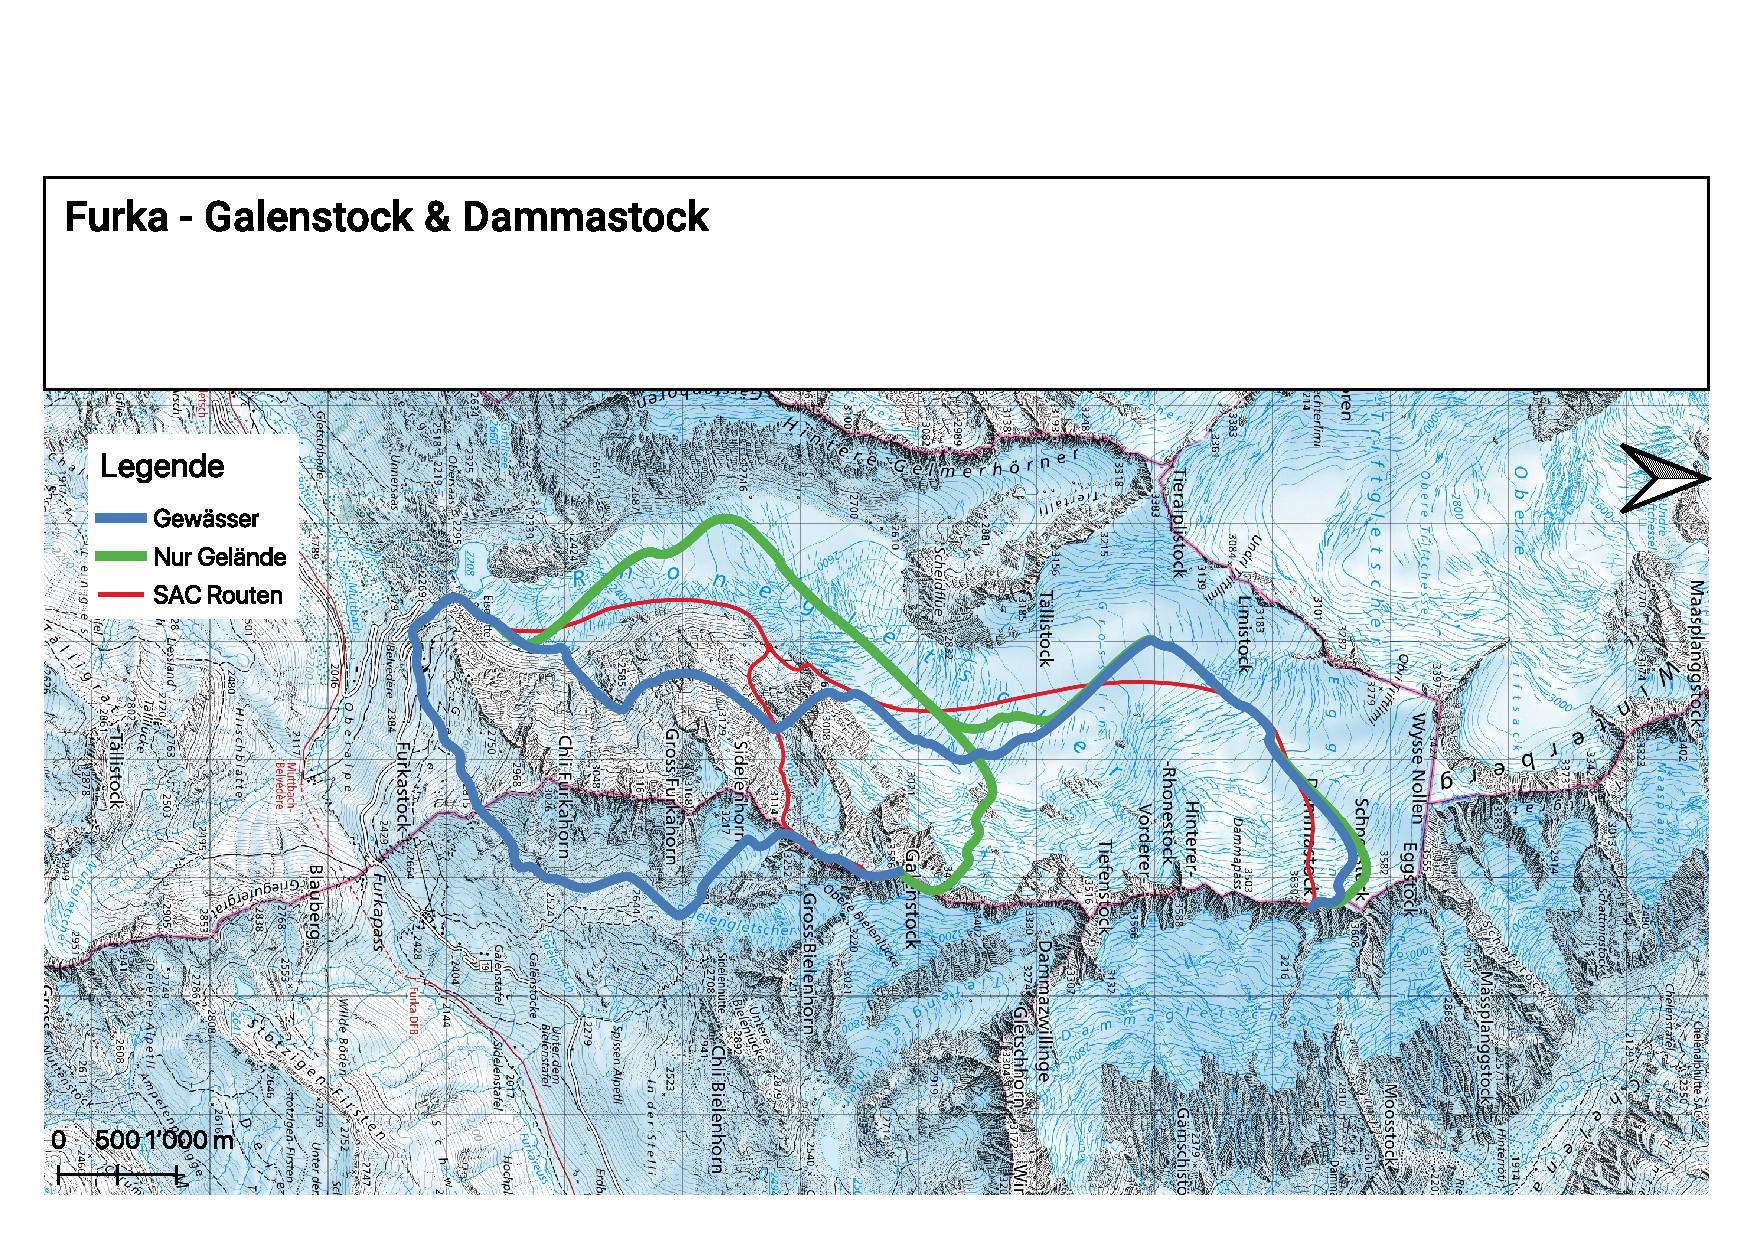
\includegraphics[page=1,width=.9\linewidth]{./../evaluation/PDFs/Furka - Galenstock & Dammastock.pdf}
  \caption{Geplante Tour auf Galen- und Dammastock\\Basislayer: swisstopo}\label{fig:pizpalu}
\end{figure*}
\begin{figure*}[ht]
  \centering
  \includegraphics[page=1,width=.9\linewidth]{./../evaluation/PDFs/Länta - Rheinwaldhorn_Adula.pdf}
  \caption{Geplante Tour von der Läntahütte auf das Rheinwaldhorn\\Basislayer: swisstopo}\label{fig:pizpalu}
\end{figure*}

% % \begin{multicols}{2}
Auch bei den Touren auf den Galenstock sowie den Dammastock werden eher einer Hochtour entsprechende Spurwahlen getroffen, wobei die Resultate des gewässerunterstützten Modells ungültig sind. 
In der Praxis sind diese Touren mit Skiern mangels einer attraktiven Abfahrt vom Skidepot aus keine Trendtouren-Kandidaten. Hier zeigt sich, dass das Modell nicht zwischen Ski- und Fussaufstieg unterscheidet. Es könnte sinnvoll sein, das Modell um einen Mechanismus zur Schätzung eines Skidepots bzw.\ von Tragepassagen zu ergänzen. Eine solche Funktionalität ist in\ \citeauthor{footandcautionsection} beschrieben und hat sich als praktikabel erwiesen~\cite{footandcautionsection}. Im gleichen Zug wäre eine automatische Schätzung der Schwierigkeit in der Skitourenskala des \acrshort{sac} denkbar. 
Alle Routen werden im Anhang\ \ref{app:evalroutes} zusätzlich gross abgebildet.

% \end{multicols}
\clearpage

\subsection{Einschränkungen des Modells}
Die vom Modell verwendete Reduktionsmethode entspricht de facto der \acrshort{grm}. So übernimmt diese primär auch deren Schwächen. Es existiert mit der quantitativen Reduktionsmethode eine Methode, welche ein umfassenderes Bild des Geländes betrachtet.~\cite{qrm}
Leider lassen die Quellen keine vollständige Reproduktion zu.

Das Modell leidet grundsätzlich unter einem Zielkonflikt. In der aktuellen Implementation kann das Modell theoretisch entscheiden, einen zu 100\% tödlichen Abschnitt zu durchqueren, wenn die Wegersparnis gross genug ist. In der Praxis ist dies jedoch selten der Fall und wurde während der Evaluation nie beobachtet.

Ist ein Grat im \acrshort{dhm} genügend breit verzeichnet, wird dieser momentan mit einem Risikowert nahe von $0.00$ ausgewiesen, ungeachtet der tatsächlichen Begehbarkeit. Hier gilt das Prinzip <<garbage in, garbage out>>. Die Datengrundlage lässt keine schlüssige Aussage über die Begehbarkeit von Graten zu.

Weiter erlaubt SwissTLM\textsuperscript{3D} keine Aussage zur Breite und Durchquerbarkeit eines Fliessgewässers, bzw.\ zur Frage, ob dieses im Winter zufriert.

\subsection{Mögliche Verbesserungen}\label{sec:improvements}

Das Potenzial des Computers wird bei der Erstellung von Risikokarten bisher nur unzureichend genutzt. Eine komplexere Reduktionsmethode als die \acrshort{grm} ist daher wünschenswert. Vielversprechende Alternativen sind beispielsweise die \gls{qrm}, die derzeit auf der Plattform skitourenguru.com eingesetzt wird, sowie SLABS, ein bisher nur theoretisch erprobtes, verbessertes probabilistisches Verfahren zur Lawinenrisikobewertung~\cite{qrm}\cite{slabs}. Diese Umstellung lässt sich einfach durchführen, da in der Entwicklung dieser beiden erwähnten computergestützten Risikobeurteilungsmethoden der benötigte Quellcode bereits verfasst wurde. Dessen Veröffentlichung wäre im Rahmen der Publikation der Werke wünschenswert gewesen.

Es gilt ausserdem, eine andere Kombinationsmethode von Anstrengung und Risiko zu prüfen. Aus Zeitgründen wurde in dieser Arbeit darauf verzichtet. Momentan wird eine einfache Summe verwendet, eine Multiplikation oder ein maximales Element könnten den bestehenden Sachverhalt besser abbilden. Kein Mensch springt über eine Klippe ab, wenn dadurch Wegzeit gespart werden kann (Abseilen wird hier als Seltenheit auf Skitouren hier einmal ausgelassen).

Eine andere denkbare Erweiterung ist ein Richtungsattribut. Die Gewichtung von negativer bzw.\ positiver Vertikaldistanz könne einfach ergänzt werden. Diese Parameter bestehen bereits, sind jedoch fix auf einen Aufstieg eingestellt. So wird das Durchqueren unnötiger Mulden beispielsweise vermieden. Ebenfalls unterscheiden sich die Anforderungen an Abfahrtsgelände von jenen an Aufstiegsgelände. In der Praxis wird in der Abfahrt meist steileres Gelände bevorzugt.

Bedenkt man, wie wenig der Computer tatsächlich von Topografie versteht, ist es im Grunde genommen erstaunlich, wie gut die produzierten Routen sind. Viel mehr lässt sich, abgesehen von den oberen Verbesserungen, aus diesem simplen Modell jedoch nicht mehr herausholen. Eine nächste Version müsste verschiedene Landformen klassifizieren und entsprechend reagieren können. Lokalwissen, wie die Begehbarkeit von Graten, könnte in einem neuen Datensatz gesammelt werden. Diese Information liesse sich beispielsweise aus GPS-Tracks der Skitouren-Community ableiten. Bemühungen diese Datengrundlagen laufend zu sammeln und zu erweitern laufen bei der Skitourenguru GmbH bereits. Leider aber wird der Datensatz proprietär gehalten. Das Erfassen dieser Daten sprengt den Rahmen einer Maturaarbeit erheblich. Damit liessen sich die Probleme betreffend Gratkletterei und spontanen Schwimmaktionen jedoch lösen.  Eine manuelle Selektion in der Nutzeroberfläche wäre als mögliche Erweiterung denkbar.

\clearpage
\subsection{Anwendungsbereich}

Aus diesen Beobachtungen lassen sich Interpretationsrichtlinien ableiten:
Im Schema 3$\times$3 siedelt sich das Modell als Ausgangslage der Stufe \textbf{Regional} an -- gleich wie ein Tourenführer. Grundsätzlich sollte mit jeder Route, egal welchen Ursprungs, kritisch umgegangen werden~\cite{sacbergspwinter}. Die endgültige Spuranlage, die Stelle von Spitzkehren oder ob ein Einzelhang wirklich durchquert wird liegt in der Entscheidungsgewalt des jeweiligen Tourengängers. So wäre es sinnvoller, gemäss \citeauthor{eisenhuttourknopfdruck} <<Korridore>> anstelle von Ideallinien vorherzusagen~\cite{eisenhuttourknopfdruck}. So kann die Unsicherheit des Modells besser vermittelt sowie ein kritischer Umgang mit dessen Ausgabe gefördert werden. Alternativrouten sollten in jedem Fall in Betracht gezogen werden. Falls eine Route sich im Gelände als unplausibel herausstellt, kann eine andere, im Voraus festgelegte Richtung eingeschlagen werden.

% \begin{multicols}{2}
\clearpage
\addtocontents{toc}{\protect\newpage}
\section{Methodische Reflexion}
\subsection{Versionsverwaltung, Backup und Archiv mit Git}

In der Softwareentwicklung haben sich Softwareversionierungstools wie \code{git} bereits bewährt. Mit diesen ist es möglich, laufende Veränderungen in Textdateien (bzw. Programmcode) zeitlich sortiert zu speichern. So kann auf verschiedenen Rechnern an unterschiedlichen Versionen gearbeitet werden, welche anschliessend mit minimalem Aufwand wieder zusammengeführt (gemerged) werden können. Jede Änderung wird als <<Commit>> gespeichert -- diese können mit einem kleinen Kommentar versehen werden. Man ist ausserdem frei darin, auf einen vorherigen Commit zurückzuspringen, sollte man mit einer Änderung nicht mehr zufrieden sein. Kurz: Zeitreise für Softwareentwicklung.~\cite{chacon2014pro}
In dieser Arbeit wurde jeglicher Programmcode sowie die Arbeit selbst in ein Git-Repository <<eingecheckt>>. Dieses wurde auf GitHub synchronisiert, um ein sicheres, cloudbasiertes Speichern aller Daten zu ermöglichen und einen Arbeitsverlust zu verhindern -- was sich als absolut empfehlenswert herausgestellt hat. Speziell die Kombionation von Git und LaTeX hat sich für das Verfassen einer Arbeit als mächtige Arbeitsweise bewährt.

\subsection{Verworfene Variante}

Die erste Variante, mit der Risikokarten hätten erstellt werden sollen, stellte sich als unpraktisch heraus. Aufgrund einer Quelle wurde eine 3D-Lawinensimulation implementiert, bzw.\ ein Versuch in diese Richtung unternommen\ \cite{athmaps}. Die Physiksimulation könnte jedoch nicht korrekt implementiert werden, mangels des nötigen mathematischen Geschicks\footnote{Numerische Verfahren zur Lösung von partiellen Differentialgleichungen entziehen sich der Expertise des Autoren, Speziell Runge-Kutta-Heun konnte trotz mehrtägiger Bemühungen ohne externe Hilfe nicht erarbeitet werden.}. Mit diesem hier nur kurz ausgeführten Unterfangen liesse sich bereits eine ganze Arbeit füllen. Hier wurde der Versuch jedoch nach ca.\ einer Woche abgebrochen. In Kommunikation mit dem Entwickler wurde mir eine kostenlose Lizenz für den kommerziellen Lawinensimulator \code{RAMMS::Avalanche} zur Verfügung gestellt.

Zwischenzeitliche wurde eine Lawinensimulation mittels \code{RAMMS::Avalanche} in Betracht gezogen. Aufgrund der hohen Rechenanforderung musste die einfachere Variante, die der \gls{grm} ähnelt, ausgewählt werden. Der eigentliche Zweck der Software entspricht auch nicht der hier verlangten Anwendung. Eigentlich werden mit der Software Gefahrengutachten für Infrastrukturprojekte erstellt. Dabei werden meist grosse Lawinen- bzw. Steinschlagereignisse mit langen Wiederkehrperioden von 10 bis 300 Jahren simuliert.

\subsection{GIS}

Der Versuch mittels minimaler externer Werkzeuge zu arbeiten stellte sich schnell als mühsam heraus. Trotzdem wurde erstaunlich lange daran festgehalten. Hier hätte schneller gewechselt werden können. 
Grosse Fortschritte resultierten vor allem durch den Wechsel von rohem Python auf QGIS.\ QGIS ist speziell geeignet, da es ein quelloffenes und erweiterbares Werkzeug ist. So konnte nicht vorhandene Funktionalität einfach durch ein selbst geschriebenes Plugin ergänzt werden.
\pagebreak
\subsection{Verfassen mit LaTeX}
Bereits in meiner Projektarbeit hat sich gezeigt, dass Microsoft Word ein denkbar ungeeignetes Werkzeug zum Verfassen von Arbeiten ist. Nach kurzem Einarbeiten in die grundsätzlichen Befehle, vielen Google-Anfragen und anfänglichen Kopfschmerzen zeigte LaTeX schnell, weshalb es so weit verbreitet ist. Eine stärkere Empfehlung im <<Handbuch Projekte>> seitens der Schule wäre wünschenswert.

\subsection{Evaluation}

In der ersten Fassung des Projektvertrages sollte die Evaluation anhand von Expertenmeinungen stattfinden. Dies wurde im  Verlauf der Arbeit verworfen, da eine hohe Expertise in der Bedienung des Modells nötig ist, um brauchbare Parameter auszuwählen. Der für das Erwerben der nötigen \gls{gis}-Kenntnisse, Auswählen und Evaluieren von Routen erforderliche Zeitumfang konnte Freiwilligen nicht zugemutet werden. Nach Vorschlag der Betreuungsperson wurde schliesslich die Variante des Vergleichs mit Literaturrouten gewählt.

\subsection{3D-Karte \& Web-App}

Dank des hohen Standards, der bei der Entwicklung von MapLibre~GL~JS durch die Beitragenden eingehalten wird, konnte innert kürzester Zeit eine erste Version der 3-D-Karte erstellt werden~\cite{maplibregljs}. Swisstopo liefert ihre Grundlagenkarte <<Base-VT>> ebenfalls in einem Format, das bereits kompatibel ist. Das Grundgerüst der Web-App wurde in Vue.js implementiert, was ich während meines NAWIMAT-Praktikums erlernt habe. Diese Wahl stellte sich als sehr günstig heraus, auch wenn eine minimale Adaptionsschicht zwischen Vue und MapLibre zusätzlich implementiert werden musste.

Die grössten Schwierigkeiten stellten sich beim Umwandeln der Höhendaten. Diese mussten von GeoTIFF in ein sogenanntes RGB-\acrshort{dem} umgewandelt werden, von der Höhe als direktem Rasterwert zu einem RGB-Bild, in welchem die Höhe als Farbwert kodiert ist. Durch das Verändern der Bildgrösse treffen die neuen Pixel nicht genau auf die alten Pixel. Für Bilddaten würde man nun bilinear interpolieren, d.h. die Farbwerte der vier umliegenden Pixel je nach Distanz gewichtet verrechnen. Probiert man dies mit RGB-\acrshort{dem}-Bildern, verfälscht man die Höhen an Kanten, bei denen zum ersten Mal blaue Pixel relevant werden (es entstehen falsche, hohe Spitzen). Die Lösung für dieses eigentlich triviale Problem bestand darin, QGIS anhand einer \acrshort{cli}-Flag mitzuteilen, nur das nächste Pixel anstelle der nächsten vier zu verwenden. Leider ist dies nicht dokumentiert und musste durch Ausprobieren herausgefunden werden.

% \end{multicols}
